\documentclass[aps,pra,notitlepage,amsmath,amssymb,letterpaper,12pt]{revtex4-1}
\usepackage{amsthm}
\usepackage{graphicx}

%  Helpful commands to set up problem environments easily
\newenvironment{problem}[2][Problem]{\begin{trivlist}
\item[\hskip \labelsep {\bfseries #1}\hskip \labelsep {\bfseries #2.}]}{\end{trivlist}}
\newenvironment{solution}{\begin{proof}[Solution]}{\end{proof}}

% --------------------------------------------------------------
%                   Document Begins Here
% --------------------------------------------------------------

\begin{document}

\title{CW 1}
\author{Kaiqin Huang}
\affiliation{CS 510}
\date{\today}

\maketitle




\begin{problem}{Derivative}
What is the definition of the derivative $f'(x)$?
\end{problem}

\begin{solution}
It means the rate of change of function $f(x)$.

\begin{equation}
\frac{df(x)}{dx} = \text{lim}_{\Delta{x}\rightarrow0}\frac{f(x+\Delta{x})-f(x)}{\Delta{x}} \nonumber
\end{equation}




Here is an explanation by figure.

\begin{figure}[h!] % h forces the figure to be placed here, in the text
  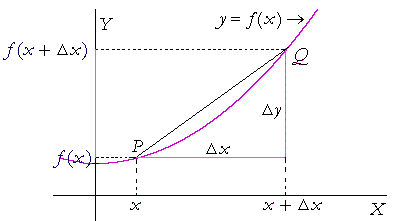
\includegraphics[width=0.4\textwidth]{007b.png}  % if pdflatex is used, jpg, pdf, and png are permitted
  \caption{Derivative (Source: Google search)}
%  \label{Source: Google search}
\end{figure}




Derivative is also the slope of the tangent line as showed above.

This text should be below the figure unless \LaTeX decides that a different layout works better.
\end{solution}
 
% Repeat as needed
 
 
\end{document}
%sagemathcloud={"latex_command":"pdflatex -synctex=1 -interact=errorstopmode 'testlatex.tex'"}